% Chapter 1

\chapter{TDSE Solution \& Optimisation} % Main chapter title

\label{Chapter3} % For referencing the chapter elsewhere, use \ref{Chapter1} 

%----------------------------------------------------------------------------------------


\section{Time Evolution of a Quantum State}
\subsection{Exact Solutions and Limitations}
The evolution of a quantum state can be described fully by the Schr$\ddot{o}$dinger equation, in it's time-dependent form, which we will refer to from now as the TDSE. The TDSE states that an arbitrary quantum state, $\Psi$, will evolve according to;
$$ 
i \hbar \frac{\partial}{\partial t} \Psi=H \Psi,
$$
where H is the Hamiltonian of the system, and is in general also time-dependent. We now consider the case where the Hamiltonian does not evolve with time - this is a much easier case to solve, in fact only a few particular systems with non-constant Hamiltonians are analytically solvable. We will investigate these numerically later in this chapter.

Solving this equation, we obtain 
$$
\Psi\left(t\right) = e^{\frac{i}{\hbar}Ht}\Psi\left(0\right),
$$
where a constant of integration has been neglected as it amounts to a global phase-shift.

By spectrally decomposing $\Psi$ into it's component eigenstates, $\sum_{i}{c_{i}\mathbf{e_{i}}}$, we can rewrite this as;
$$
\Psi\left(t\right) = \sum_{j}{e^{\frac{i}{\hbar}\lambda_{j}t}c_{j}\mathbf{e_{j}}\left(0\right)},
$$
allowing us to see that each individual eigenstate oscillates in amplitude, with a frequency determined by the energy of the eigenstate.

Solutions for this case can therefore be exactly calculated if the eigenstates are known, and so we can use this case to compare to our numerical model solutions to measure their accuracy.

\subsection{The Case for Numerical Methods}
The TDSE is not trivially solvable analytically other than for particular time-dependent Hamiltonians; and so to be able to investigate the time evolution of more complicated systems, or systems with more complicated external potentials, a different approach must be used. 

One alternative approach is pertubation theory, where known solutions to Hamiltonians of simpler systems are used to approximate the more complicated systems along with small additional `perturbative' terms. This approach's accuracy is mostly limited by the size of the pertubation, and so is useful for modelling the evolution for systems similar to an analytically solvable one with a small additional term - but not in the general case for modelling arbitrary systems.

Another approach is to use numerical methods; discretizing the Hamiltonian and wavefunction and using numerical solutions to the differential equation by approximating derivatives with series or basis expansions - as we did for the numerical solutions to the TISE. 

Advantages of this approach include that computers are easily able to compute solutions to discretized models, and that these approaches are not limited to systems similar to analytically solvable ones - as they do not rely on the solutions to the differential equation being similar, instead solving the differential equation in a completely different way.

In this chapter we investigate and compare two numerical methods of solving the TDSE; a Finite Difference propagator, and a Krylov Subspace propagator. These both work similarly, using one or more previous states of the wavefunction to predict the state at the next timestep, and updating the Hamiltonian at ever timestep.

\section{Finite Difference Propagator}
A finite difference approach to this problem is very similar to the one used in solving the TISE - with the main difference being that we are now propagating in time rather than space. Additionally, as we don't know anything about the wavefunction at points in time ahead of the current timestep, we can't use any backwards terms in our finite difference scheme. 

FD methods require knowledge of the wavefunction at several initial timesteps to be able to start to propagate; in the TISE solution we took the initial points to be all $0$, but that is an unsuitable assumption for this case. 

Instead, we use analytic solutions to the field-free case to build up the first few timesteps. This is equivalent to assuming that no external potential is applied to the system for the first few timesteps, which is a much more realistic assumption.

\section{Krylov Subspace Propagator}
The Krylov Subspace approach works differently, calculating the state of the wavefunction at the next timestep in terms of only the current one. 

To do this, a krylov subspace is built from a matrix representation of the Hamiltonian at the next timestep and using the current wavefunction as the starting vector for the subspace. 

The vectors in the subspace are then added, weighted by appropriate taylor series coefficients, to give the approximation for the wavefunction at the next timestep. This approximation increases in accuracy with increased subspace size, although almost all information is contained in the first few terms and there is a rapidly decreasing benefit to additional subspace elements - the rate of the descrease here is considerably greater than the decrease in benefit of using additional finite difference terms in the FD propagator case. However, the computational costs of using more terms are not the same in both propagators and so it is non-trivial to determine which method is more efficient in any given case - this will be discussed later in this chapter.

To summarise the process;
First the Krylov subspace, $\mathbb{K}$, is built:
$$
\mathbb{K} = \left[\Psi\left(t\right) ,\ H\left(t+\delta{t}\right)\Psi\left(t\right) ,\ H^{2}\left(t+\delta{t}\right)\Psi\left(t\right) ,\ ... \right]
$$
Then a weighted sum of the subspace elements, $\{k_{i}\}$, is used to approximate $\Psi\left(t+\delta{t}\right)$:
$$
\Psi\left(t+\delta{t}\right) = \sum_{i}{\frac{-i\delta{t}^{i}}{i!}k_{i}}
$$

Advantages of this approach include accurate convergence with relatively few terms needed, and that there is no need for the first few terms to be analytic solutions to the field-free case.
Disadvantages of it include that a large matrix-vector multiplication must be performed for every term in the approximation, as opposed to a single one regardless of the number of terms in the FD approach.
%This 'baseline solution' finds the first $k$ eigenstates of the Hamiltonian associated with an elecron interacting with a Hydrogenic atom at an instant, with the Coulomb Potential being modelled instead by a Soft-Core potential - which at all but very small distances is an accurate approximation of the Coulomb Potential. Due to the Coulomb Potential tending towards $\infty$ as $r\rightarrow 0$ it is difficult to model it numerically, but with a Soft-Core Potential approximation, we avoid the issues at small $r$s yet obtain accurate results for everywhere other than at the center.

\section{Comparisons Between Time Propagators}

\subsection{Efficiency Comparisons For 6000 Timesteps With A Small Grid}
Using only the constant Soft-Core potential, and so with no time-dependent terms in the Hamiltonian, the two propagators were used to propagate the Ground State wavefunction 6000 timesteps - using a 1000 grid points to represent the wavefunction, a timestep of $10^{-3}$ atomic units of time, and both propagators using 6 terms. The results shown are averaged over 5 repeated calculations. 

For context if attempting to reprodce the results, the calculations were performed in a Python3.7 Jupyter Notebook, running on a 3.2GHz i7u processor with 8GB of RAM.

\subsubsection{Krylov Subspace Propagator:}
Mean runtime: \hspace{2cm} 32.28598s\newline
Standard Deviation: 0.10144s / 0.31419\%

\subsubsection{Finite Difference Propagator:}
Mean runtime: 26.62208s\newline
Standard Deviation: 1.18747s / 4.46047\%

\textbf{Note:} It was noticed for this set of results that 4 runs were extremely close to 26s, with a single result being almost 29s. The cause of this anomaly was investigated and was determined to be that I switched to a different browser tab during that calculation; Facebook, which loads a number of videos and images when opened. The anomalous result was replaced with 3 new calculations to instead give the following results;\newline
Mean runtime: \hspace{2cm} 26.02711s\newline
Standard Deviation: 0.10275s / 0.39478\%

Additionally, I attempted to recreate the anomalous result by averaging 5 calculations during which I switched to the Facebook tab, in order to support the hypothesis that the extra compuatational power required by facebook caused the anomalous result. The results of that attempt were as follows;\newline
Mean runtime: \hspace{2cm} 33.73616s\newline
Standard Deviation: 5.19175s / 15.38927\%

\subsubsection{Analysis:}
From these results, it is clear that for this setup the Finite Difference propagator performs more efficiently - taking only around 80\% of the time as the Krylov Subspace propagator. Additionally, both propagators had a very similar spread of times taken; showing that each is roughly as reliable as the other.

\subsection{Efficiency Comparisons For 6000 Timesteps With A Large Grid}
The previous experiment was repeated, changing only the number of grid points used to 100,000. Due to the length of time required for these calculations, they were not averaged to obtain a more accurate result and determine the spread of results; instead the spread after 500 timesteps was investigated, using 5 calculations for each propagator, afterwards to provide some insight to the expected spread of results for the full 6000 timesteps.

\subsubsection{Krylov Subspace Propagator:}
Mean runtime: \hspace{2cm} 2392.27s

\subsubsection{Finite Difference Propagator:}
Mean runtime: 2093.00s

\subsubsection{Standard Deviations after 500 timesteps:}
Krylov Subspace propagator:\newline
Mean runtime: \hspace{2cm} 198.092076s\newline
Standard Deviation: 0.62765s / 0.31685\%\newline\newline
Finite Difference propagator:\newline
Mean runtime: \hspace{2cm} 172.43040s\newline
Standard Deviation: 0.58337s / 0.33832\%

\subsubsection{Analysis:}
From the standard deviations at 500 timesteps, we can expect that at the full 6000 timesteps the standard deviations for each propagator will be very small compared to the mean - and similar in magnitude, with the Finite Difference propagator possibly having a slightly larger relative standard deviation. From this, we can conclude that for a model with many grid points the Finite Difference model outperforms the Krylov Subspace model, although to less of an extent than it does with a smaller model; taking around 87\% of the time rather than 80\%.

\subsection{Efficiency Comparisons For 60,000 Timesteps With A Small Grid}
The initial experiment was repeated, using 60,000 timesteps instead of 6,000, to investigate how the model performances scale with propagation distance. 

\subsubsection{Krylov Subspace Propagator:}

Mean runtime: \hspace{2cm} 327.40101s\newline
Standard Deviation: 0.53118s / 0.16224\%

\subsubsection{Finite Difference Propagator:}

Mean runtime: \hspace{2cm} 263.82221s\newline
Standard Deviation: 0.61104s / 0.23161\%

\subsubsection{Analysis:}
Here we see that the Finite Difference propagator still only takes about 80\% of the time to run as the Krylov Subspace propagator, matching the results for the smaller number of timesteps with the same grid size. It can also be seen that the relative standard deviations of the times taken have reduced to around half of their values for the model with fewer timesteps; this would imply that the main inconsistencies were in the setup of the models, and once that is complete there is a lower level of difference.

\subsection{Accuracy Comparisons For 6000 Timesteps Over A Small Grid}
To compare the accuracies achievable with the two methods, we are limited to cases that can be exactly solved; for this purpose we compare results for modelling field-free propagation. 

The setup of the computational experiment is mostly the same as described for the first `efficiency' test, with one difference being that the timestep size of $10^{-3}$ was found to be too large for the Krylov Subspace propagator to handle, causing massive instabilities regardless of the order of the propagator. Instead, a timestep size of $10^{-4}$ was used. 

It is worth noting that the Finite Difference propagator was able to produce reliable results even for these larger timesteps and so could be more useful in some contexts than the Krylov Subspace propagator due to this. Additionally, the fact that the end results for the Krylov Subspace propagator are completely unphysical does not detract from the findings in the above efficiencies comparison; as the number of operations performed at each timestep does not depend on the magnitude of the timestep in any way, and the number of timesteps used was kept constant.

Initially sixth-order propagators were used for each method and the accuracy is measured by comparing the population of the Ground State, i.e. the Ground State coefficient of the spectral decomposition of the propagated wavefunction, at the end of the propagation. 

Given that we use the ground state as our wavefunction, and there is no external field to excite the system, the population of the ground state should remain 1 throughout the propagation - the magnitudes of any increases or reductions to this would indicate numerical errors.

\subsubsection{CASE 1 - dt = $10^{-4}$, Grid Size = 1000, End Time = 0.6, propagation order = 6}
Krylov Subspace Error: 1.1102230246251565e-16\newline
Finite Difference Error: 2.220446049250313e-16  

\subsubsection{CASE 2 - dt = $10^{-4}$, Grid Size = 1000, End Time = 6, propagation order = 6}
Krylov Subspace Error: 0.0\newline
Finite Difference Error: -2.220446049250313e-16 

\subsubsection{Analysis:}
From these, it is clear that both are very accurate models. For clarification on the repeated result for the Finite Difference propagator, and for the fact that the first Krylov Subspace propagator result is exactly half that of the Finite Difference ones, the wavefunction is stored internally as an array of double precision floating point numbers - which have a maximum precision of -2.220446049250313e-16. Therefore the accuracy of the results are seemingly limited more by their storage medium than the fact that they are only approximations of the solution. 

Because of this, in order to determine which method is more accurate compared to the other, we must either reduce the number of terms used by each propagator or greatly increase the `end time' of the propagation.

\subsubsection{CASE 3 - dt = $10^{-4}$, Grid Size = 1000, End Time = 0.6, propagation order = 3}
Krylov Subspace Error: 3.775724177756956e-10\newline
Finite Difference Error: 0.0

\subsubsection{CASE 4 - dt = $10^{-4}$, Grid Size = 1000, End Time = 6, propagation order = 3}
Krylov Subspace Error: 3.775721957310907e-10\newline
Finite Difference Error: 1.1102230246251565e-16 

\subsubsection{Analysis:}
These results show that even when using half the number of terms in the propagators the FD method can retain accuracy to within the maximum possible tolerance of the storage medium - this was unexpected as it was believed that while the first few terms in a Krylov subspace should contain almost all of the information about the wavefunction at the next timestep, the same was not expected to be true of the FD method. One reason the FD method could be more accurate at a lower propagation order in this case is that we are investigating the ground state which is relatively smooth over the entire interval. 

Additionally, while less accurate than the FD propagator, the Krylov Subspace approach was still very accurate - and retained the accuracy when moving from the 6,000 timesteps case to the 60,000 case. This shows that the model is stable, i.e. does not contain terms that cause it to reduce in accuracy over time.

The FD propagator was further tested to failure, in order to determine how large of a timestep it could handle and still remain accurate. It was found that, with 3rd order propagation, after 6,000 timesteps it was still accurate to around machine precision for a timestep of $5e^{-3}$, for $6e^{-3}$ it had an error of 6.54306e-07, and for $7e^{-3}$ it had an error of $1$. This shows that, while it is extremely accurate and stable for small timesteps, it rapidly loses stability if the timestep is even slightly too large.

Additionally this shows that in order to approximate the wavefunction at a given time to a given tolerance, the FD approach can use both a smaller number of terms and a larger timestep - this results in orders of magnitude fewer calculations needing to be performed, allowing it to be calculated much more quickly.


For both of these propagators the critical magnitude of the timestep before instability depends on the size of the gap between grid points. We investigated this by repeating the experiments using a larger number of grid points over the same interval (100,000 vs. 1,000). As it has already been shown that either instabilities will cause the error to quickly grow, or the error will remain fairly constant during propagation if the model is stable, we only need to compare the errors after a relatively small number of timesteps in order to determine the accuracy of the model. For this purpose, we will propagate for only 300 timesteps.

\subsubsection{CASE 5 - dt = $10^{-4}$, Grid Size = 100000, End Time = 0.03, propagation order = 6}
Krylov Subspace Error: -103435.8494626187\newline
Finite Difference Error: 0.9999999999723448 

\subsubsection{CASE 6 - dt = $10^{-5}$, Grid Size = 100000, End Time = 0.003, propagation order = 6}
Krylov Subspace Error: 0.8971347740628693\newline
Finite Difference Error: 4.440892098500626e-16

\subsubsection{CASE 7 - dt = $10^{-7}$, Grid Size = 100000, End Time = 0.00003, propagation order = 6}
Krylov Subspace Error: 0.9999999999999252\newline

\subsubsection{CASE 8 - dt = $10^{-8}$, Grid Size = 100000, End Time = 0.000003, propagation order = 6}
Krylov Subspace Error: 4.440892098500626e-16\newline

\subsubsection{Analysis:}
Here we can see that when we use more grid points we need to decrease the size of the timestep to maintain stability. We see that for a grid 100 times the size, we need to decrease the the size of the timestep by around 2 orders of magnitude for the FD propagator to achieve stability, while the Krylov Subspace propagator needs the timestep to be decreased by around 4 orders of magnitude. From this we can conclude that the accuracy and stability of the solutions scale more effectively with the FD propagator than the Krylov Subspace propagator as the number of grid points increases.

\subsection{Summary of Findings}

\section{Parallelisation of the Time Propagation}
We have seen in this chapter that, assuming stability conditions are met and enough propagation terms are used, either propagator can give results at a very high level of accuracy at even distant times - with the largest limit on accuracy coming from the number of spatial grid points used to model the wavefunction. Therefore, to increase the overall accuracy we need to use a more accurate spatial representation with more grid points. 

However, as seen in the above `efficiency' comparisons, our time propagation speeds do not scale well with increased spatial grid size. 

To try to reduce this problem as much as possible, the propagators were parallelised - allowing different chuncks of the wavefunction to be propagated separately on different computers/processors/cores. 

To do this, both the wavefunction and the Hamiltonian were split into `chunks' - this is equivalent to considering the time evolution of subrergions of our interval seperately, and so they can be recombined afterwards to re-form the full evolved wavefunction. A diagram describing this process is shown below;



\subsubsection{Is Any Information Lost When The Propagation Is Split Up?}
In short, yes, although the amount can be mitigated through a few different methods. The reason we lose information, or accuracy, is that by splitting up the spatial region we introduce new boundaries in the system at the edges of the chunks. These boundaries effectively force the wavefunction to drop to 0 at any distance past the edge of the chunk, although this itself is not important as at distances past the chunk's edge the next chunk is simply used instead. What is important is that during propagation, the wavefunction inside each chunk thinks the rest of the wavefunction is 0-valued - this causes `reflections' at the boundaries, which cause inaccuracies at the edges of the chunks and can start to cause inaccuracies further and further within the chunk over time. 

The figure below shows an example of this; where the wavefunction was split into two equally sized chunks, propagated seperately for 1000 timesteps, then recombined. It can be seen that there are large differences from the expected result at the centre, but elsewhere a very accurate result is obtained.



These `reflections' should actually occur even for the non-parallelised case, except that in this case the assumption that the wavefunction is 0-valued beyond the edges is actually a good assumption and closely approximates the physical system. From the description of the cause of these reflections, it can be seen that the impact of these reflections depend on how far from 0 the wavefunction should be at the boundaries - for example, in the above figure we have that the chunk boundaries are at the peak of the wavefunction, and so this is a worst-case scenario. We now consider methods of mitigating the errors introduced by these reflections.

\subsection{Avoiding Problems At Chunk Edges}
As mentioned previously, there are several approaches to limiting or avoiding the errors introduced by reflections. One such method is to share knowledge of the values of a few spatial points of the chunked wavefunctions with their neighbouring chunks after every few timesteps; allowing the neighbours to re-adjust their wavefunction based on this knowledge - this is the approach used in RMT, which we will see in more detail in Chapter 5. A diagram describing this process is given below;



Limitations of this method include that requiring communication between chunks is costly, and limits the advantage of parallelisation as the subprocesses can no longer operate fully independently. For example, if the propagation was split across three computers, one of which was far slower than the other two and information about edge points was shared every 10 timesteps; although each computer would only need to perform one third of the total number of calculations, the two fast computers are only able to calculate up to 10 timesteps further before being stalled to wait for the third computer. If information did not need to be shared, the two fast computers could complete their calculations without needing to wait for the third. 

This cost can be limited, by either ensuring all computers perform similarly or by varying the size of the chunks to match the performance of the comuter propagating them such that they can all propagate their chunk at around the same speed. The communication of edge information between computers itself also has an associated computational cost, which cannot be as easily limited.


Another method of avoiding problems at the edges of chunks is to `overlap' chunks. If, for example, 10 extra spatial points are given to each chunk on either side - and knowing that after propagation the errors caused by reflections mostly affect the outermost spatial points, then the next most outermost, and so on - then provided we haven't propagated far enough for the reflections to permeate too deeply into the wavefunction chunk the errors are almost entirely confined to the outer 10 spatial points. As these were `extra' points we stuck on to each chunk, we can simply discard their values, then recombine the remainder of our chunks to form the full wavefunction with the errors caused by reflections almost entirely ignored. 

The process described is explained in the diagram below;



In the event that we want to propagate further in time, the errors caused by reflections will come further inside the chunked wavefunction. We can avoid this by increasing the number of spatial points used in the overlap, although this will increase the computational cost of propagation. 

Limitations of this method include that extra calculations (in the overlapped regions) need to be performed, increasing the overall computational cost, and these costs only increase with further time propagation meaning it does not scale well for large end times. However, relatively few overlap points are needed to mitigate most of the errors, and the there is an exponential decay on the impact of reflection errors as you move further from the edges - and so the rate of increase of the number of extra spatial points needed to propagate to the end time reduces as the end time grows. 

An advantage this approach has over the last is that no communication is needed between the chunks; due to this there is no additional communication cost, and the wavefunction and Hamiltonian can be split into more chunks than there are computers - reducing the amount of work needed to propagate each chunk and allowing any faster computers to immediately start working on the next chunk upon completion of a chunk propagation, rather than waiting for the propagation of the other chunks to finish first.

\subsection{Efficiency Testing}
ARCHER (* CITE *) define several quantities; `Speed-Up' ($S$), `Parallel Efficiency' ($E_{\text{par}}$), and `Serial Efficiency' ($E_{\text{ser}}$) which we will use to evaluate the effectiveness of our parallelisation. These quantities are defined in terms of execution time, $T$.
\begin{itemize}
	\item[-]{\textbf{Speed-Up: }
		$$
		S\left(N,P\right) = \frac{T\left(N,1\right)}{T\left(N,P\right)}
		$$}

	\item[-]{\textbf{Parallel Efficiency: }
		$$
		E_{\text{par}}\left(N,P\right) = \frac{S\left(N,P\right)}{P} = \frac{T\left(N,1\right)}{PT\left(N,P\right)}
		$$}

	\item[-]{\textbf{Serial Efficiency: }
		$$
		E_{\text{ser}}\left(N\right) = \frac{T_{\text{best}}\left(N\right)}{T\left(N,1\right)}
		$$}
\end{itemize}
Where $N, P$ are the size of the problem and number of processors respectively.

Amdahl (* cite archer *) stated in 1967 that "The performance improvement to be gained by parallelisation is limited by the proportion of the code which is serial". Effectively, this means that a given process can be approximated by a part or parts that is non-parallelisable and a part or parts that are; and so even with the best parallelisation scheme the process will take at least as long as the non-parallelisable parts take to run. 

He exteds this concept into `Amdahl's law'; given a process that has a fraction, $\alpha$, that is completely serial and that the rest is a perfectly efficient parallel scheme, we can describe the parallel runtime and speedup as follows:
$$
T(N, P)=\alpha T(N, 1)+\frac{(1-\alpha) T(N, 1)}{P}\\
S(N, P)=\frac{T(N, 1)}{T(N, P)}=\frac{P}{\alpha P+(1-\alpha)}
$$

From these, we can see that a parallel scheme will only be worthwhile if the serial part, $\alpha$, is small. 

To properly investigate the benefit of our parallel scheme, we need to investigate both the Parallel and Serial Efficiencies. This was performed on a server cluster, AIGIS (node aigis11), which has 32 available cores - each capable of running 2 threads and with a clock speed of 2.3GHz. 

\subsubsection{Parallel Efficiency}
The parallel efficiency of our setup was investigated by timing the propagation of a wavefunction with 50,000 spatial grid points 10,000 timesteps, using between 1 and 32 cores. The following results were obtained;

\begin{figure}[H]
         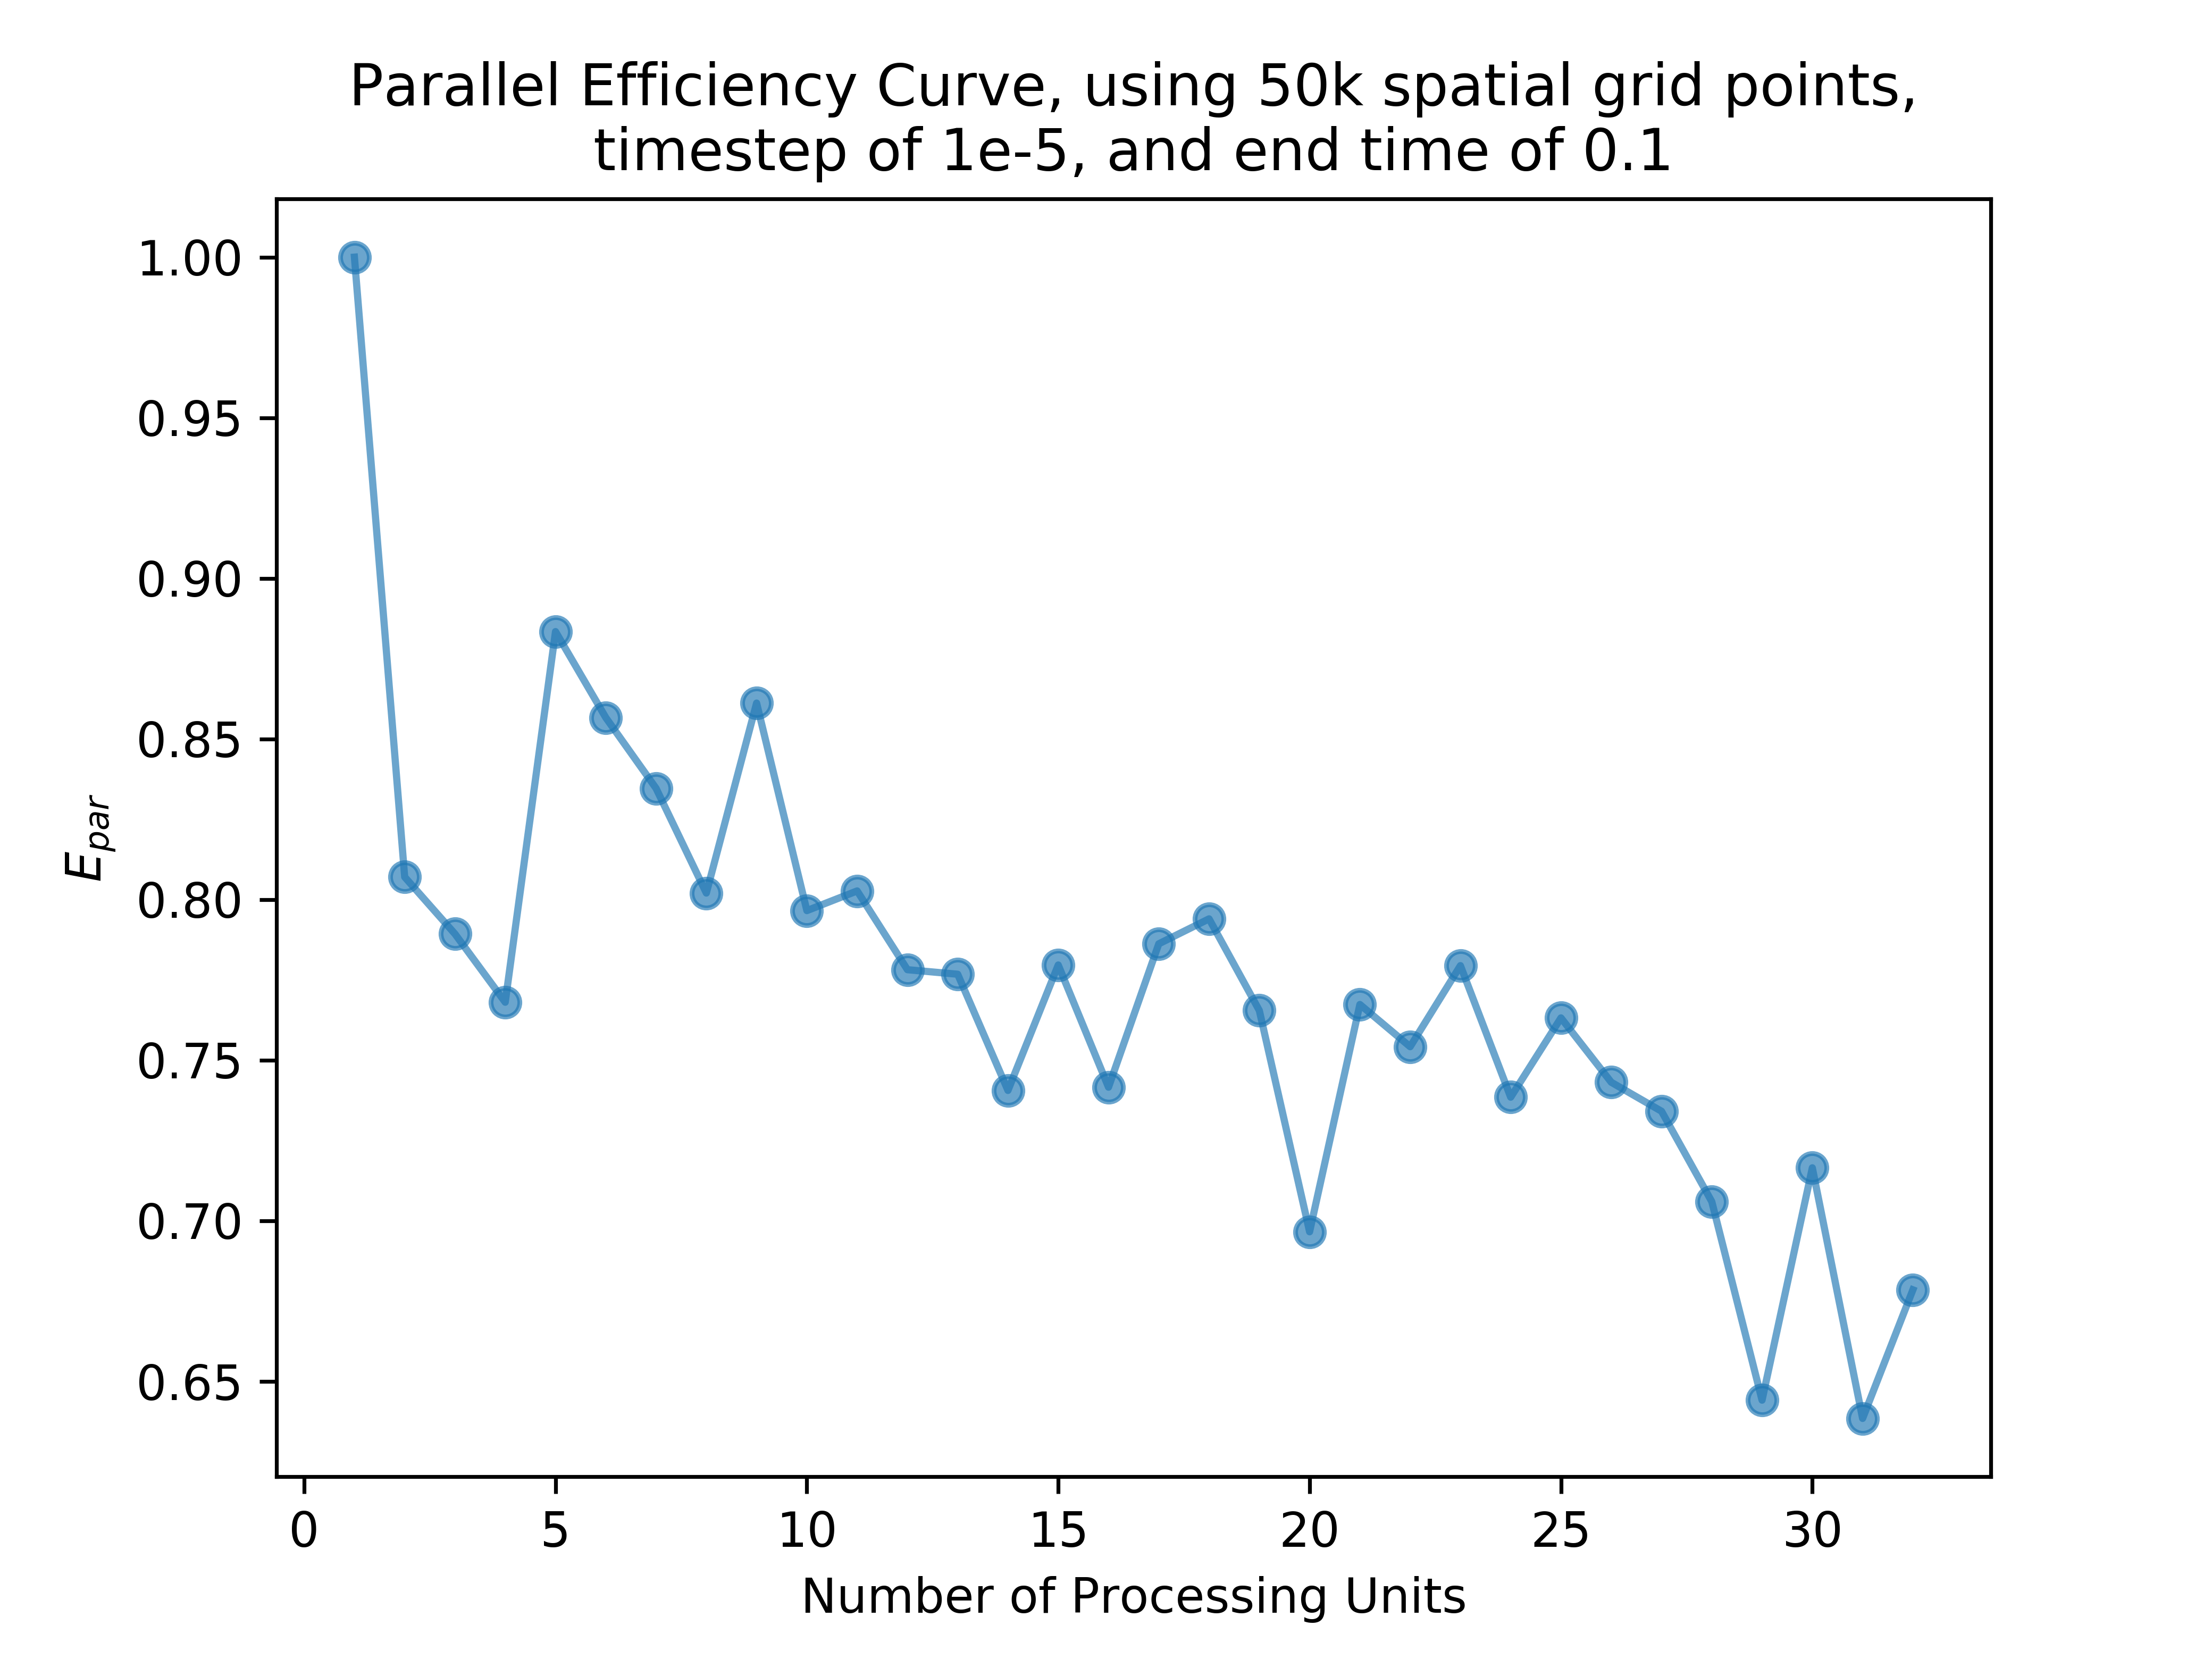
\includegraphics[width=\textwidth]{./ParEffCurve.png}
         \centering
         \caption{Parallel Efficiency Curve}
\end{figure}


Figure <x> shows that the rate of speedup for our scheme falls as the number of additional processors increases, although only a little; from the first additional processor to the thirty-first additional one, we only see an efficiency drop of around 0.2. So although there is a reducing amount of benefit from each additional processor, scheme still performs well on our server cluster - as it is limited to 32 cores, and our scheme has a reasonable benefit from each additional core even until all available cores are used here.

\subsubsection{Serial Efficiency}
The serial efficiency of our parallelised model was investigated by timing the propagation of a wavefunction with between 250 and 41,000 spatial grid points for 10,000 timesteps using both our `best' parallelisation scheme and the non-parallelised scheme. I took the `best' scheme to be the case where we use 31 cores, as it performed very similarly to when using the full 32 cores and as it was less likely to be interupted if anyone else started a job on the same node at the same time. The graph below describes the resuts;

\begin{figure}[H]
         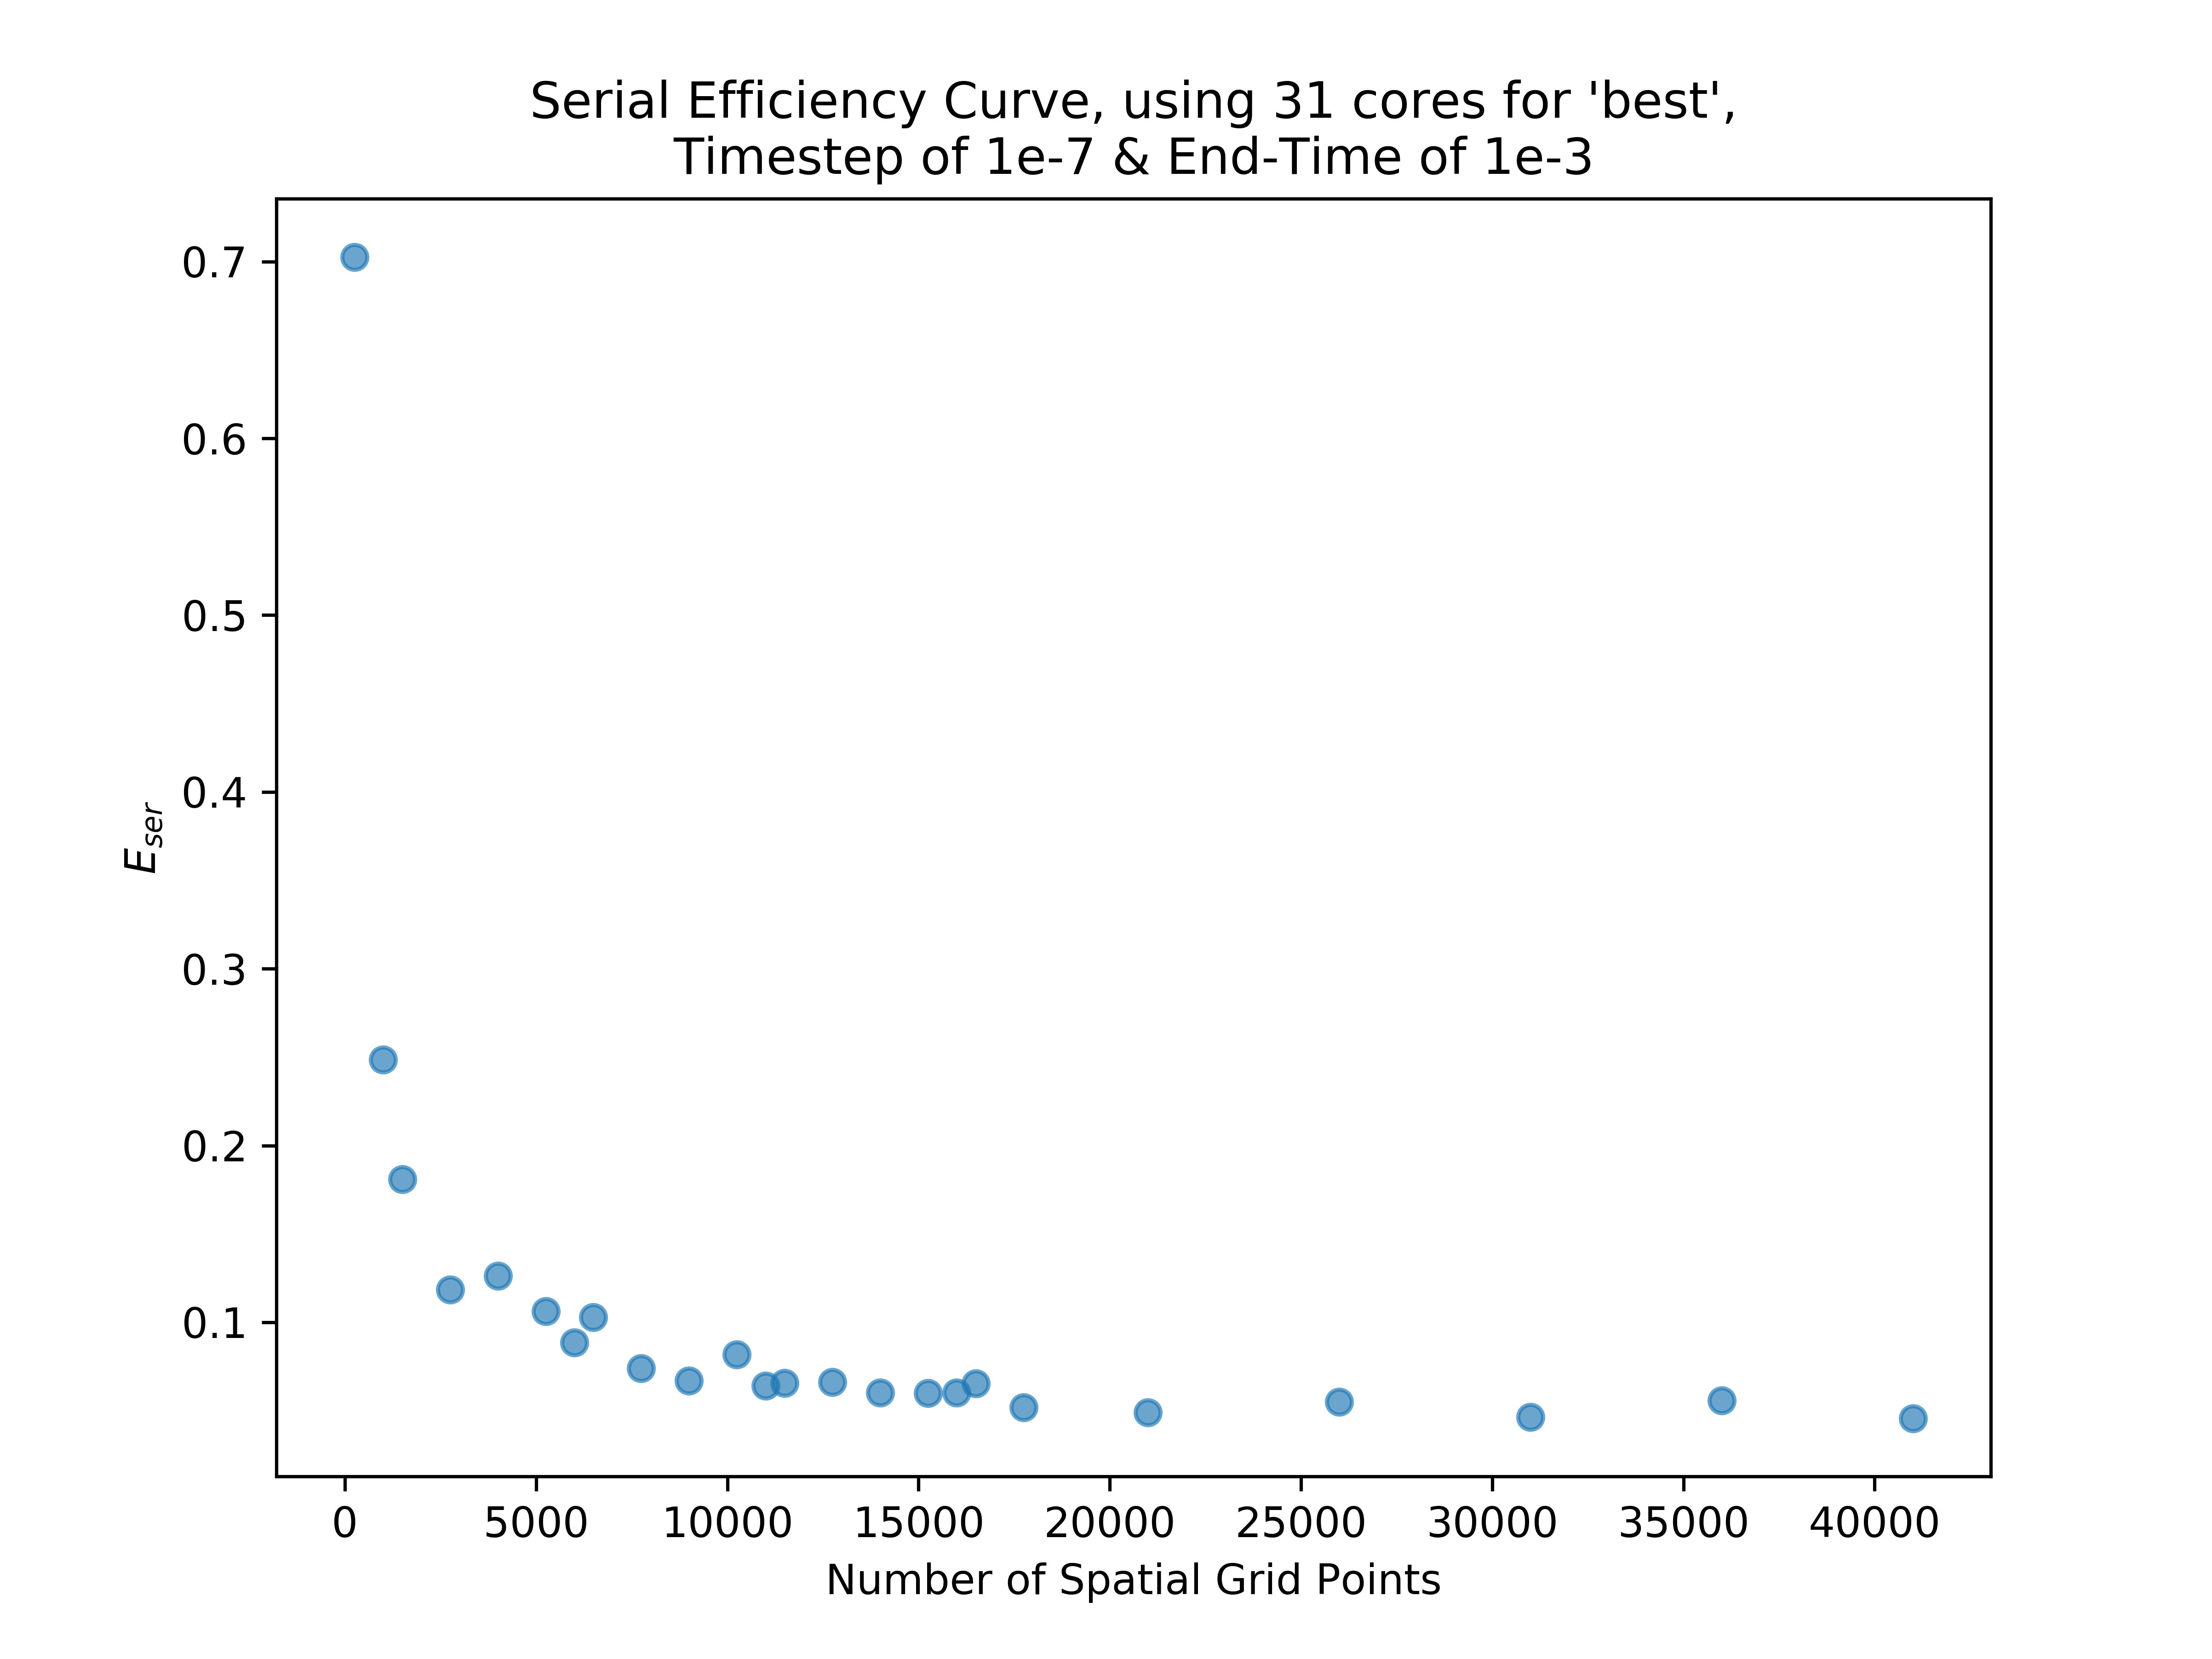
\includegraphics[width=\textwidth]{./SerialEff.png}
         \centering
         \caption{Serial Efficiency Curve}
\end{figure}



Figure <x2> shows an increasing benefit ratio to using the parallelised scheme as the number of grid points grows, but this ratio converges at 17500 spatial grid points - after which the benefit ratio is fairly constant at around 0.04, showing that this scheme caps out at being around 25x faster than the non-parallelised version no matter how many additional processing units are given.

\subsubsection{Comments}
%----------------------------------------------------------------------------------------

